\usetikzlibrary{arrows,positioning}
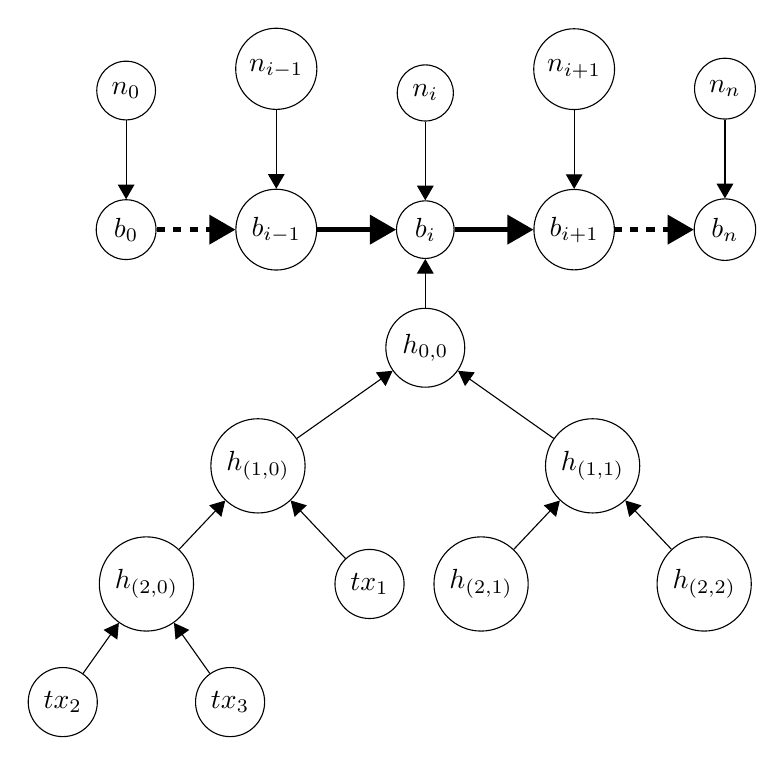
\begin{tikzpicture}[level/.style={sibling distance=85mm/#1}, 
                                    every node/.style={circle,draw},
                                    every path/.style={<-,>=triangle 60}]
\node (bi) {$b_i$}
child {node (h00){$h_{0,0}$}
  child {node (h10) {$h_{(1,0)}$}
    child {node (h20) {$h_{(2,0)}$}
      child {node (t2) {$tx_2$}}
      child {node (t3) {$tx_3$}}
    }
    child {node (h20) {$tx_1$}}
  }
  child {node (h11) {$h_{(1,1)}$}
    child {node (h21) {$h_{(2,1)}$}}
    child {node (h22) {$h_{(2,2)}$}}
  }
};

\node[left=of bi] (biminus) {$b_{i-1}$} edge[->,ultra thick] (bi);
\node[right=of bi] (biplus) {$b_{i+1}$} edge[<-,ultra thick] (bi);

\node[left=of biminus] (b0) {$b_0$} edge[->,dashed,ultra thick] (biminus);
\node[right=of biplus] (bn) {$b_n$} edge[<-,dashed,ultra thick] (biplus);

\node[above=of b0] (n0){$n_0$}edge[->] (b0);
\node[above=of biminus] (n0){$n_{i-1}$}edge[->] (biminus);
\node[above=of bi] (n0){$n_{i}$}edge[->] (bi);
\node[above=of biplus] (n0){$n_{i+1}$}edge[->] (biplus);
\node[above=of bn] (n0){$n_{n}$}edge[->] (bn);

\end{tikzpicture}